\section{Konzept}
\label{btc_konzept}
Die folgenden Schritte beschreiben den Finanzfluss zwischen den Teilnehmern und der Anwendung, sowie die Gewinnerauswahl durch den in der Zukunft liegenden Blockchain-Status. Der Ablauf ist allgemein gehalten und kann nicht nur mit Bitcoin, sondern auch mit anderen Kryptowährungen, die auf einer Proof-of-Work Blockchain basieren, umgesetzt werden. Betrachtet wird ein Spiel mit $N \in \{2,5,10\}$ Teilnehmern, bei dem jeder Teilnehmer einen Einsatz von $X$ Währungseinheiten zur Teilnahme zahlen muss. 

\begin{enumerate}
\item Im ersten Schritt eröffnet die Anwendung ein neues Spiel in dem es $N$ freie Plätze und einen leeren Geldtopf gibt.
\item Sobald ein Spieler am Spiel teilnehmen möchte, generiert die Anwendung eine neue Empfangsadresse\footnote{Man könnte auch allen Spieler die gleiche Einzahlungsadresse anzeigen. (siehe Abschnitt \ref{sssec:Auszahlungstransaktion})} und zeigt diese dem Spieler an.
\item Der Spieler verwendet die Wallet Software seiner Wahl um eine Transaktion zu erstellen, die den Einsatz an die angezeigte Empfangsadresse überweist. Die Wallet Software signiert die Transaktion und leitet sie über die mit ihr verbundenen Nachbarknoten an das Peer-to-Peer Netzwerk weiter.
\item Sowohl die Anwendung als auch die Miner empfangen die Transaktion. Die Anwendung zeigt dem Nutzer über die GUI an, dass die Transaktion zwar erhalten wurde, allerdings noch nicht bestätigt wurde. Die Miner des Netzwerks nehmen die Transaktion in ihren nächsten Block auf.\footnote{Natürlich nur unter der Annahme, dass sie die Höhe der Transaktionsgebühr als angemessen empfinden.}
\item Ein Miner findet den zu seinem Block passenden Proof-of-Work-Hash und schickt den Block an das Netzwerk.
\item Die Applikation empfängt den Block und merkt, dass im Block eine Transaktion auf die in Schritt 2 generierte Empfangsadresse enthalten ist. Die Applikation prüft die Höhe des Transaktionsbetrags und leitet anschließend die vom Spieler kontrollierte Auszahlungsadresse aus der Transaktion ab. 
\item  Die restlichen $N-1$ Teilnehmer überweisen ebenfalls den geforderten Betrag auf die ihnen angezeigte Empfangsadresse.
\item  Sobald die letzte Transaktion in einen validen Block aufgenommen wurde, zählt die Reihenfolge in der die Transaktionen in der Blockchain stehen. Die Reihenfolge steht somit fest und kann nicht mehr nachträglich verändert werden. Der Geldtopf ist nun mit einem Betrag von $N*X$ Krytowährungseinheiten gefüllt und wird geschlossen. Der Nachfolger des Blocks, in dem die letzte Einzahlungstransaktion eingegangen ist, wird zur Gewinnerauswahl genutzt. Die Anwendung merkt sich die Blocknummer dieses Blocks.
%\item Die Anwendung signiert nun die Reihenfolge der Teilnehmer und deren Auszahlungsadressen und schreibt die resultierende Signatur mit einer Transaktion in die Blockchain.
\item Die Anwendung und die Teilnehmer warten darauf, dass der nächste Block von einem Miner gefunden wird. Alle Miner des Peer-to-Peer Netzwerks versuchen schnellstmöglich einen passenden Blockhash zu finden, um den Blockreward zu erhalten. Ein Miner gewinnt dieses Rennen und teilt dem Netzwerk den neu gefundenen Block mit.
\item Die Anwendung empfängt den nächsten Block und ermittelt durch diesen den Gewinner. Die Berechnung erfolgt auf Basis der letzten Ziffer\footnote{Man kann an dieser Stelle auch den gesamten Blockhash als Grundlage der Gewinnerauswahl nehmen. Die daraus resultierenden Vor- und Nachteile werden in Abschnitt \ref{btc_gewinnerauswahl} erörtert.} $d_{last}$ des Blockhashs in Hexadezimaldarstellung. Durch die Berechnung von $d_{last}$  modulo $N$ resultiert eine Zahl $G \in \{0,...,N-1\}$, die den Gewinner festlegt. Der Spieler, der die $G+1$te Einzahltransaktion gesendet hat, gewinnt den Geldtopf\footnote{Es handelt sich zu diesem Zeitpunk erst um den vorläufigen Gewinner des Spiels, da es zu einem Blockchain Fork (siehe Abschnitt \ref{sssec:btc_fork}) kommen kann. }.
\item Sobald die Anwendung einen Block empfängt, der auf den Block für die Gewinnerauswahl aufbaut, beginnt die Auszahlung des Gewinns. Die Anwendung erstellt dazu eine neue Transaktion, die alle $N*X$ Krytowährungseinheiten des Geldtopfs an die Auszahlungsadresse des Gewinners überweist und sendet diese an das Netzwerk.
\item Die Wallet Software des Gewinners, empfängt die Transaktion und informiert ihn darüber, dass er den gesamten Betrag des Topfes erhalten hat.
\end{enumerate}

%%%%%%%%%%%%%%%%%%%%
% Bitcoin Beispiel %
%%%%%%%%%%%%%%%%%%%%
\vspace{0.75cm}
\noindent Im folgenden Beispiel wird ein Topf mit 5 Teilnehmern, die Kryptowährung Bitcoin und einen Einzahlungsbetrag von 0,1 Bitcoin betrachtet. Dieses Beispiel verdeutlicht sowohl die Interaktion der verschiedenen Teilnehmer des Peer-to-Peer Netzwerks, als auch die Veränderung des Status der Blockchain.

\vspace{1cm}
\begin{minipage}{0.55\textwidth}
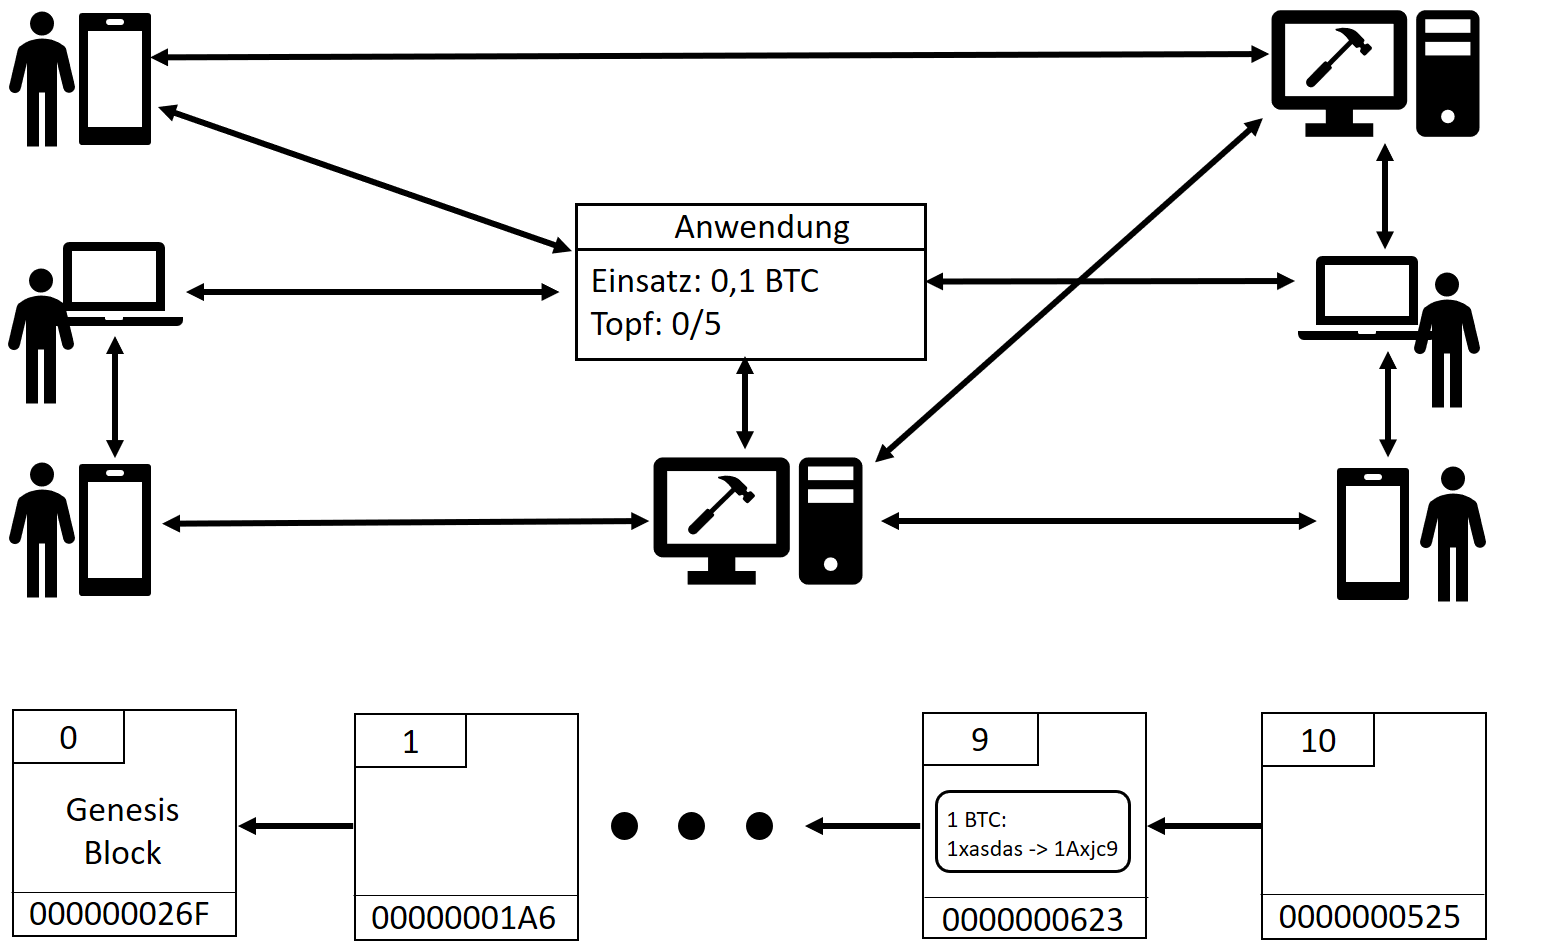
\includegraphics[width=\textwidth]{Figures/konzept_btc/konzept1}
\centering
\decoRule
\captionof{figure}{Schritt 1}
\label{fig:konzept1}
\end{minipage}
\begin{minipage}{0.45\textwidth}
Diese Abbildung zeigt das Peer-to-Peer Netzwerk. Die 5 potentiellen Teilnehmer sind durch Notebooks und Smartphones dargestellt. Außerdem sind 2 Miner und die Glücks\-spiel\-anwendung Teil des Peer-to-Peer Netzwerks. Der aktuelle Status der Blockchain, die jeder Teilnehmer des Netzwerks lokal speichert, ist unterhalb des Netzwerks dargestellt.
\end{minipage}

\vspace{1cm}
\begin{minipage}{0.55\textwidth}
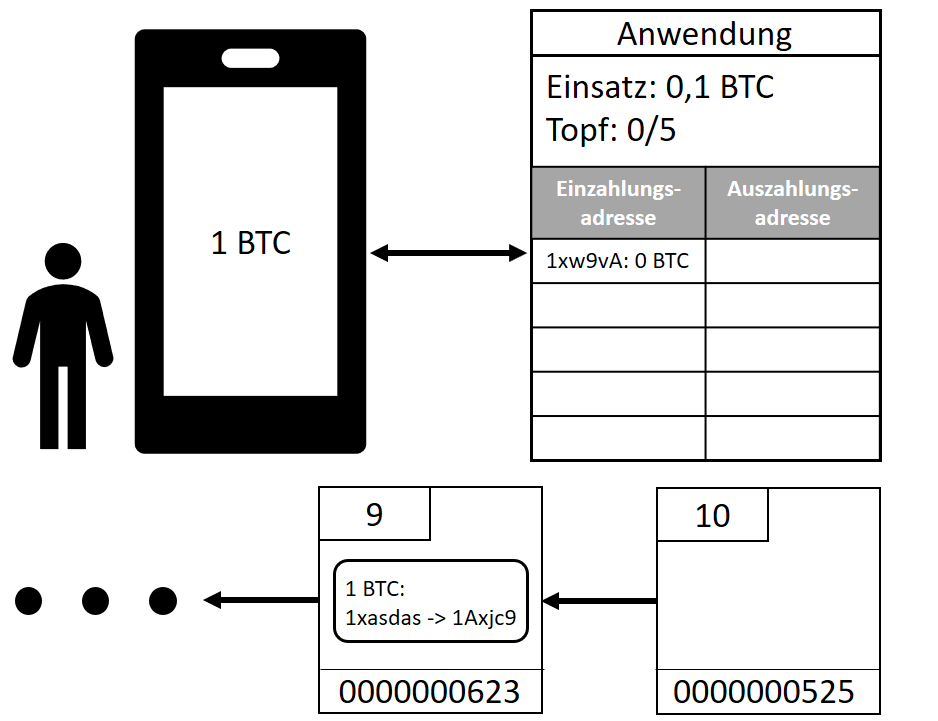
\includegraphics[width=\textwidth]{Figures/konzept_btc/konzept2}
\centering
\decoRule
\captionof{figure}{Schritt 2}
\label{fig:konzept2}
\end{minipage}
\begin{minipage}{0.45\textwidth}
Die Bitcoin Client Software der Glücksspielanwendung generiert eine neue Bitcoinadresse und speichert den dazugehörigen privaten Schlüssel in der Wallet. Sobald Bitcoins auf dieser Adresse empfangen werden, können sie nur durch den Besitz des privaten Schlüssels weiter transferiert werden.
Die Anwendung zeigt dem Benutzer eine frisch generierte Empfangsadresse über die Benutzeroberfläche an. Der Zustand der Blockchain verändert sich nicht.
\end{minipage}

\vspace{1cm}
\begin{minipage}{0.55\textwidth}
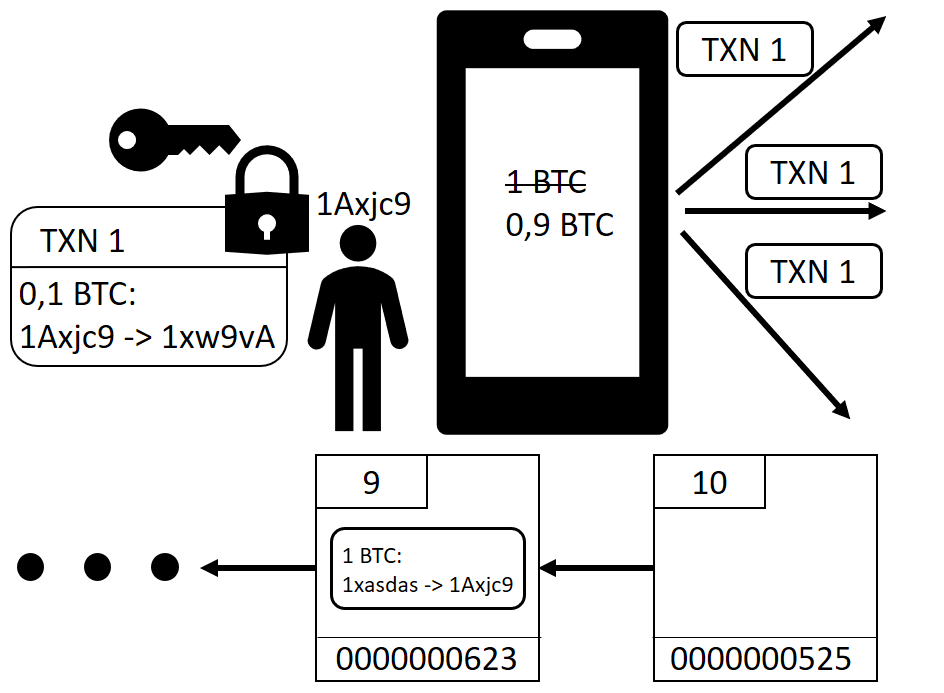
\includegraphics[width=\textwidth]{Figures/konzept_btc/konzept3}
\centering
\decoRule
\captionof{figure}{Schritt 3}
\label{fig:konzept3}
\end{minipage}
\begin{minipage}{0.45\textwidth}
Nun zahlt der Spieler mithilfe seiner Bitcoin Wallet Software in den Geldtopf ein. Dazu erstellt er eine Transaktion (TXN 1), die Bitcoin von seiner Adresse auf die generierte Adresse der Glücksspielanwendung transferiert. Durch die Signierung mit seinem privaten Schlüssel autorisiert er die Überweisung. Anschließend schickt er die Transaktion seinen Nachbarknoten.
\end{minipage}

\vspace{1cm}
\begin{minipage}{0.55\textwidth}
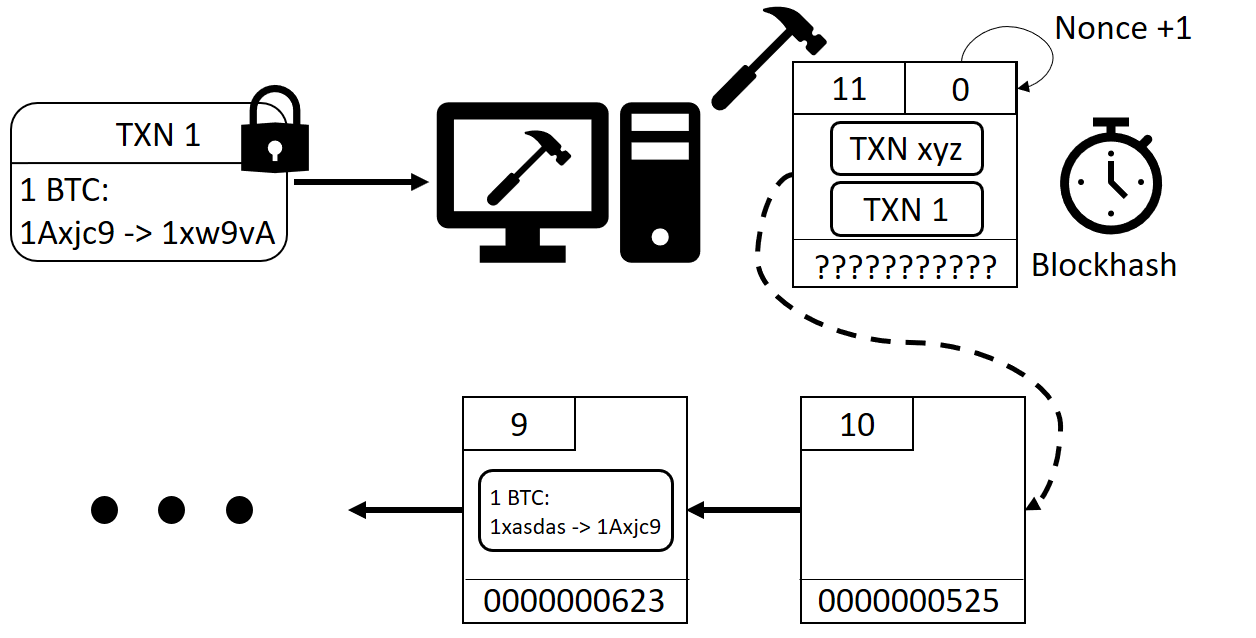
\includegraphics[width=\textwidth]{Figures/konzept_btc/konzept4}
\centering
\decoRule
\captionof{figure}{Schritt 4}
\label{fig:konzept4}
\end{minipage}
\begin{minipage}{0.45\textwidth}
Sobald die Transaktion TXN 1 einen Miner erreicht, prüft dieser, ob die Transaktion in Einklang mit den Konsensregeln ist. In diesem Beispiel existiert in Block 9 eine Transaktion von einem Bitcoin auf die Adresse des Teilnehmers. Unter der Annahme, dass dieser Bitcoin nicht in Block 10 weiter überwiesen wurde, befindet sich auf der Adresse des Teilnehmers somit ein Bitcoin. Außerdem prüft der Miner ob die Signatur der Transaktion gültig ist. Da die Transaktion valide ist, fügt er sie dem aktuell zu generierenden Block Nummer 11 hinzu. 
\end{minipage}


\vspace{1cm}
\begin{minipage}{0.55\textwidth}
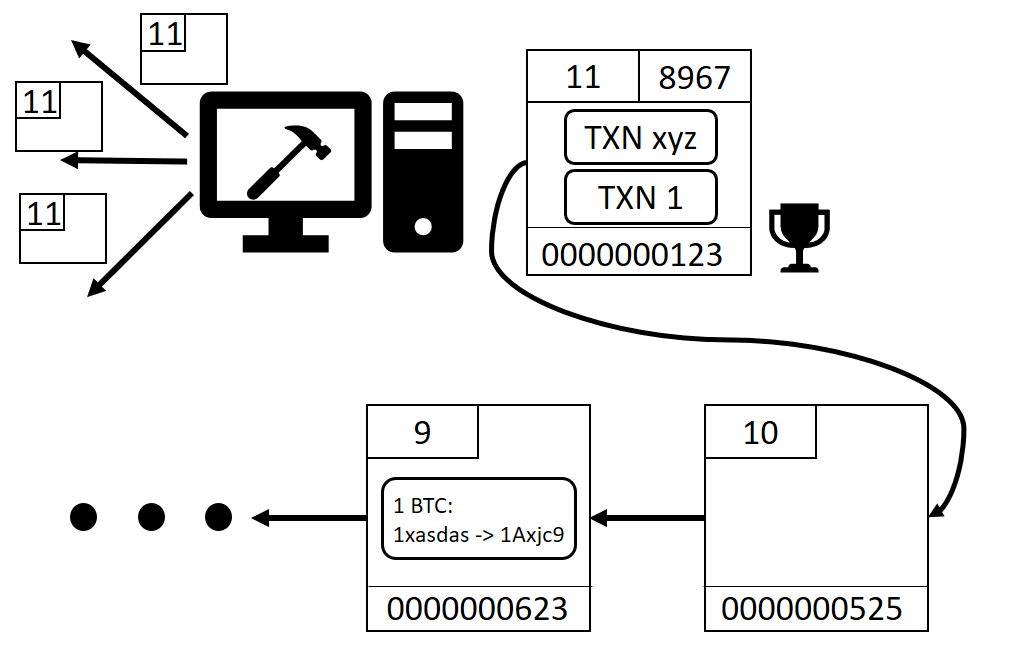
\includegraphics[width=\textwidth]{Figures/konzept_btc/konzept5}
\centering
\decoRule
\captionof{figure}{Schritt 5}
\label{fig:konzept5}
\end{minipage}
\begin{minipage}{0.45\textwidth}
Der Miner berechnet nun mithilfe der Hashfunktion den Hash des Blocks. Falls der Blockhash-Wert den durch die Konsensregeln dynamischen angepassten Schwierigkeits-Wert unterschreitet, gilt der Block als valide. Überschreitet der Blockhash den Wert erhöht der Miner den Nonce-Wert des Blocks und berechnet den Blockhash erneut. Diesen Prozess wiederholt er solange bis er entweder einen gültigen Blockhash findet oder einen gültigen Block Nummer 11 von einem anderen Netzwerkteilnehmer empfängt.
In diesem Beispiel findet der Miner einen gültigen Blockhash, leitet den Block an das Netzwerk weiter und wird dadurch mit neu erschaffenen Bitcoin für seinen Rechenaufwand belohnt.
\end{minipage}

\vspace{1cm}
\begin{minipage}{0.55\textwidth}
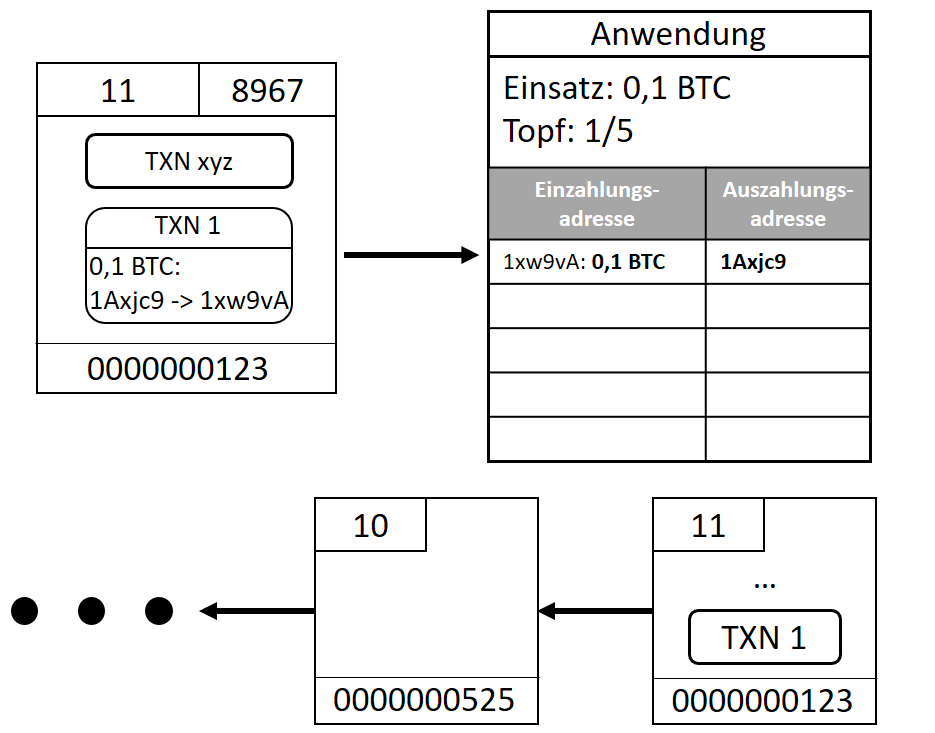
\includegraphics[width=\textwidth]{Figures/konzept_btc/konzept6}
\centering
\decoRule
\captionof{figure}{Schritt 6}
\label{fig:konzept6}
\end{minipage}
\begin{minipage}{0.45\textwidth}
Die Glücksspielanwendung empfängt den Block Nummer 11 und überprüft, ob er im Einklang mit den Konsensregeln ist. Dies ist der Fall. Somit wird die lokale Blockchain Datenbank um einen Block erweitert. Die Glücksspielanwendung hat somit den Einsatz des ersten Spielers erhalten. Sie zeigt nun die vorher noch unbestätigte Transaktion als bestätigt an und fügt den Spieler zum Topf hinzu. Aus der Einzahlungstransaktion des Spielers leitet die Anwendung die Auszahlungsadresse \textbf{1Axjc9} des Spielers ab. 
\end{minipage}

\vspace{1cm}
\begin{minipage}{0.55\textwidth}
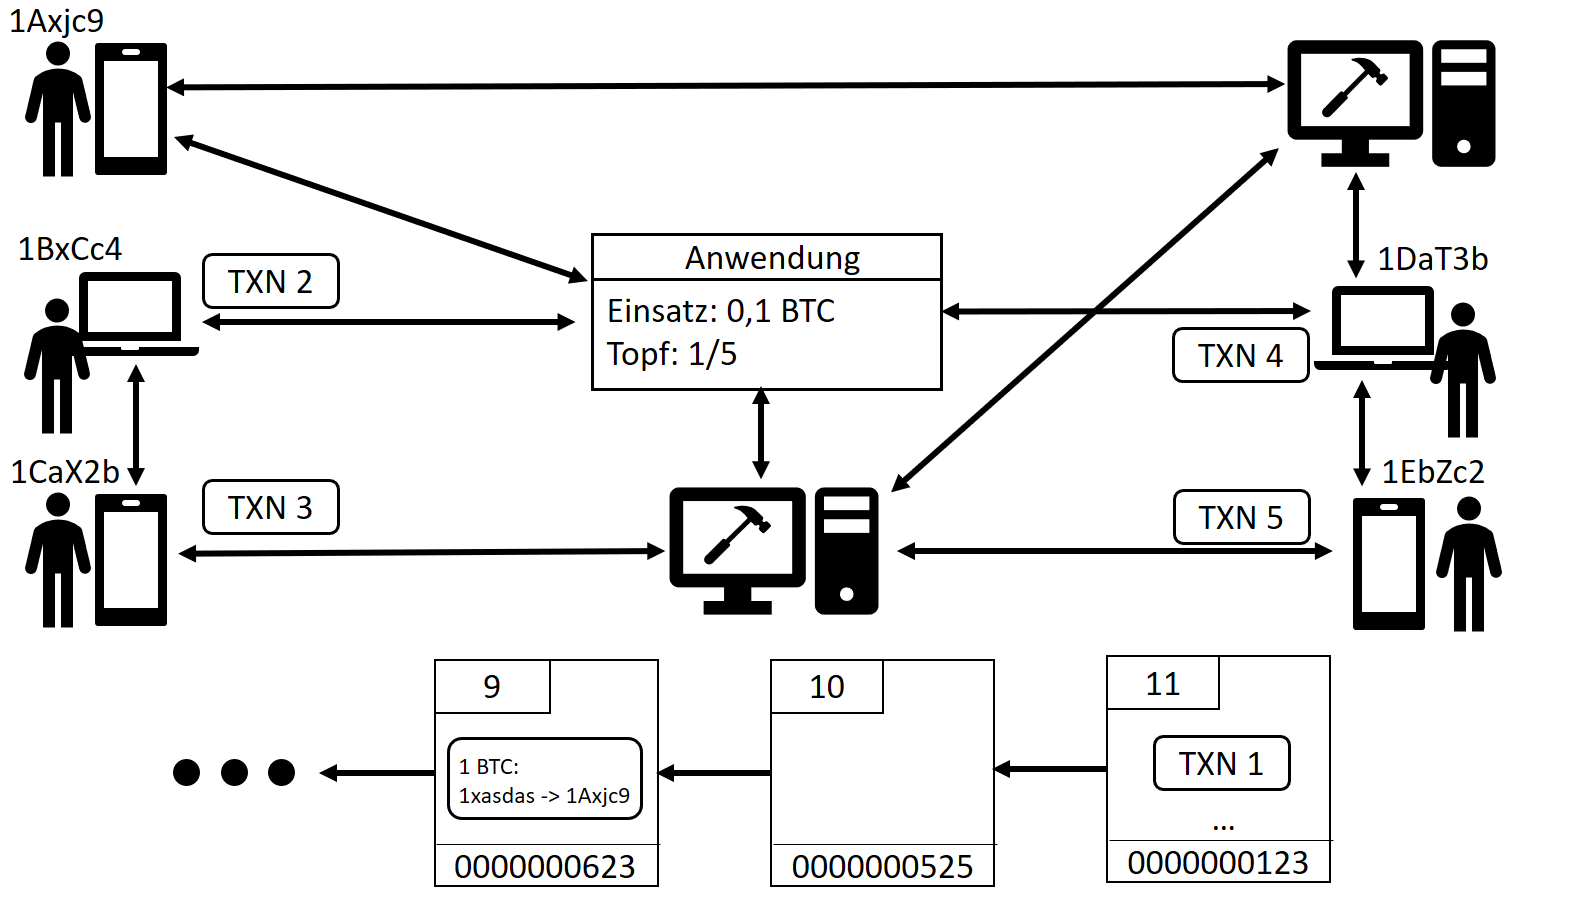
\includegraphics[width=\textwidth]{Figures/konzept_btc/konzept7}
\centering
\decoRule
\captionof{figure}{Schritt 7}
\label{fig:konzept7}
\end{minipage}
\begin{minipage}{0.45\textwidth}
Die restlichen Spieler senden ihre signierten 0,1 Bitcoin Transaktionen in das Peer-to-Peer Netzwerk. Diese sind in Abbildung 7 durch die Transaktionen TXN 2 bis 5 dargestellt.
\end{minipage}

\vspace{1cm}
\begin{minipage}{0.55\textwidth}
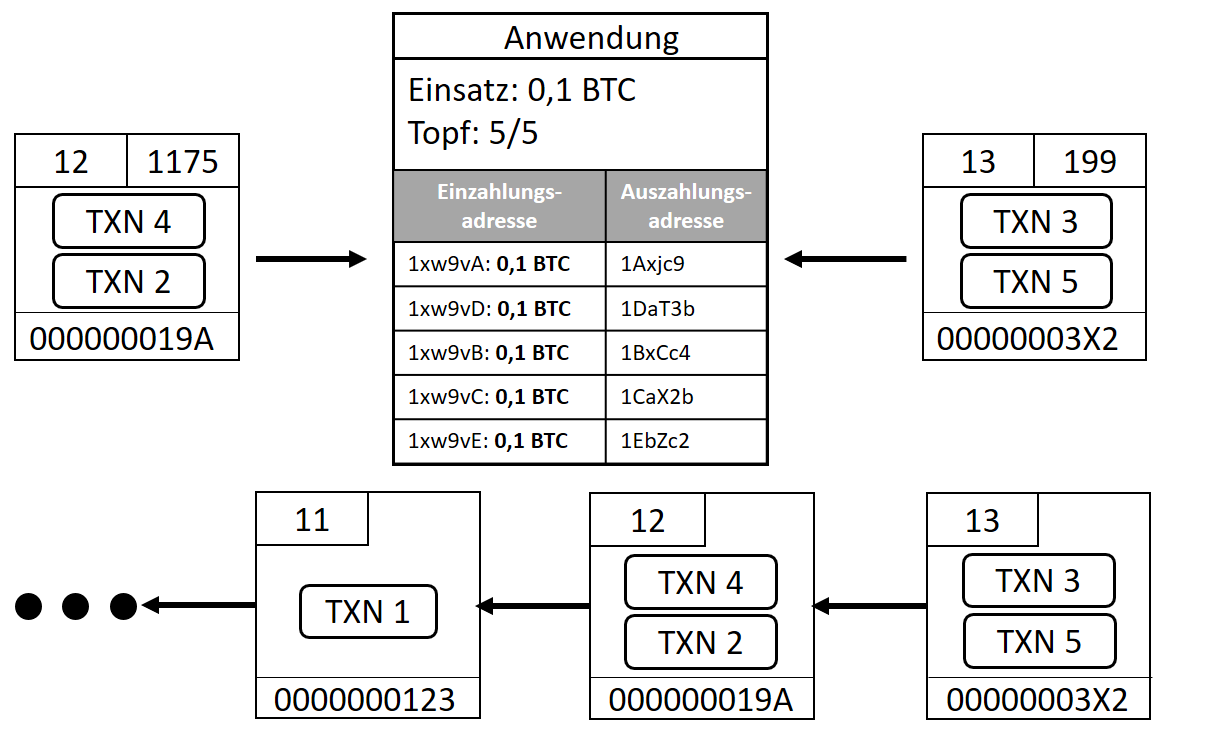
\includegraphics[width=\textwidth]{Figures/konzept_btc/konzept8}
\centering
\decoRule
\captionof{figure}{Schritt 8}
\label{fig:konzept8}
\end{minipage}
\begin{minipage}{0.45\textwidth}
Beliebige Miner fügen die Transaktionen in ihre Blöcke ein. Sobald die Glücksspielanwendung die Blöcke empfängt, prüft sie diese gegen die Konsensregeln und fügt sie in die lokale Blockchain ein.
Die Applikation merkt nun, dass alle Spieler bezahlt haben und schließt den Geldtopf. Dabei merkt sie sich die Nummer des Blocks, in dem die letzte Einzahlungstransaktion vorhanden ist. Der darauffolgende Block mit Nummer 14 wird für die Ziehung des Gewinners verwendet.
\end{minipage}

\vspace{1cm}
\begin{minipage}{0.55\textwidth}
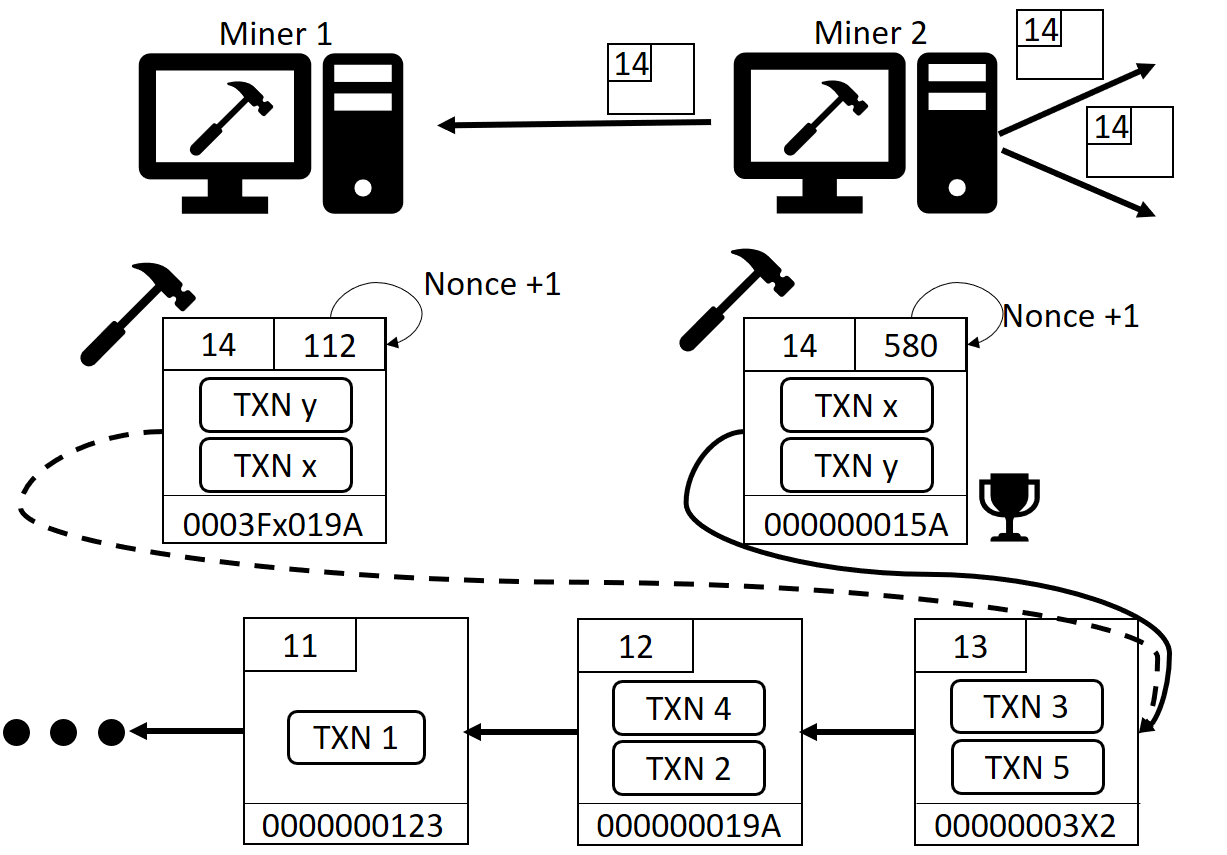
\includegraphics[width=\textwidth]{Figures/konzept_btc/konzept9}
\centering
\decoRule
\captionof{figure}{Schritt 9}
\label{fig:konzept9}
\end{minipage}
\begin{minipage}{0.45\textwidth}
Alle Miner des Netzwerks versuchen nun gleichzeitig so schnell wie möglich den nächsten Block zu finden. Da sie dazu eine kryptographische Hashfunktion benutzen, bei der die Ausgabe ein unkontrollierbarer, zufälliger Wert ist, hat keiner der Miner einen direkten Einfluss auf den resultierenden Blockhash. In diesem Beispiel findet Miner 2 einen gültigen Blockhash vor Miner 1. Miner 2 leitet seinen gültigen Block Nummer 14 so schnell wie möglich an das Netzwerk weiter und erhält den Blockreward als Belohnung. Miner 1 geht leer aus.
\end{minipage}

\vspace{1cm}
\begin{minipage}{0.55\textwidth}
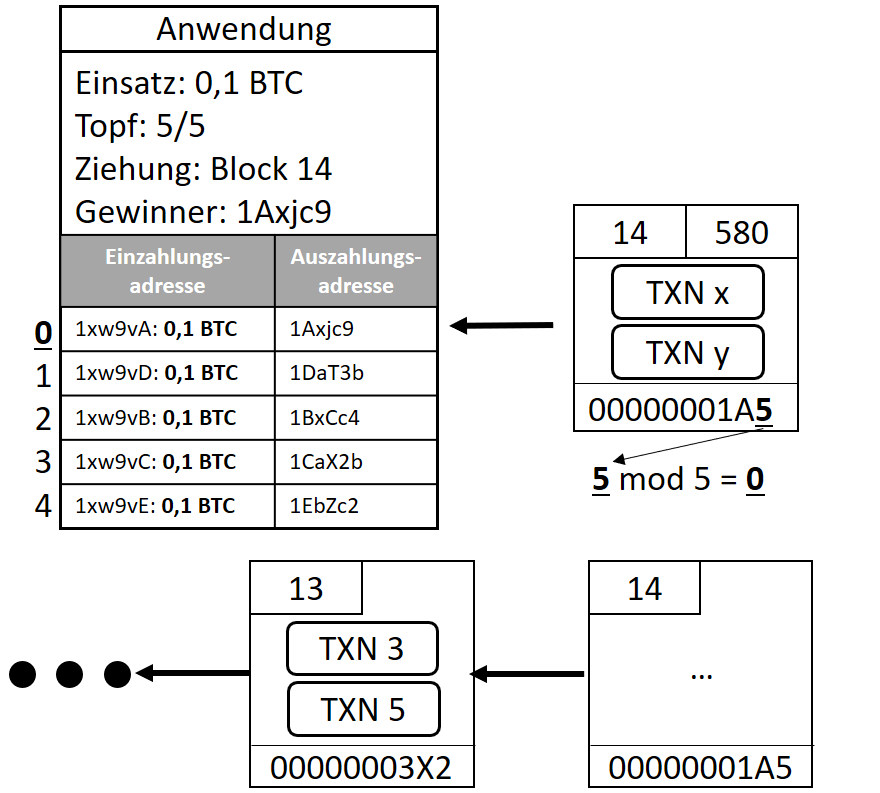
\includegraphics[width=\textwidth]{Figures/konzept_btc/konzept10}
\centering
\decoRule
\captionof{figure}{Schritt 10}
\label{fig:konzept10}
\end{minipage}
\begin{minipage}{0.45\textwidth}
Die Anwendung empfängt Block 14 und prüft ihn gegen die Konsensregeln. Der Block ist valide. Daher verwendet die Anwendung den im Block enthaltenen Blockhash um den Gewinner des Geldtopfs zu ermitteln. Statt des gesamten Blockhashs verwendet die Anwendung nur die letzte Ziffer des Blockhashs in Hexadezimaldarstellung zur Gewinnerauswahl. Dies hat den Vorteil, dass die Teilnehmer die Korrektheit der Gewinnerauswahl leichter eigenständig nachprüfen können.
Da die letzte numerische Stelle des Blockhashs 10 verschiedene Werte annehmen kann, ordnet die Anwendung jedem der 5 Teilnehmer zwei Gewinnzahlen zu.
\end{minipage}

\noindent Durch die Modulo 5 Funktion ergibt sich die Verteilung der Gewinnzahlen folgendermaßen:
\begin{itemize}
\item Spieler 1 mit Adresse 1xw9vA gewinnt bei 0 und 5,
\item Spieler 2 mit Adresse 1xw9vD gewinnt bei 1 und 6,
\item Spieler 3 mit Adresse 1xw9vB gewinnt bei 2 und 7,
\item Spieler 4 mit Adresse 1xw9vC gewinnt bei 3 und 8,
\item Spieler 5 mit Adresse 1xw9vE gewinnt bei 4 und 9.
\end{itemize}
Jeder Teilnehmer besitzt nun die gleiche Gewinnwahrscheinlichkeit\footnote{Dies gilt nur unter der Annahme, dass der Wert für die Gewinnerauswahl gleichverteilt ist. Dies wird in Abschnitt \ref{btc_distribution} genauer erläutert.} von $\frac{1}{5}$. Block Nummer 14 hat den Blockhash \textbf{000000015A}\footnote{In der Praxis ist jeder Blockhash genau 64 Zeichen lang (Hexadezimalsystem), da Bitcoin die SHA-256 Hashfunktion verwendet. Aufgrund der Länge ist es praktisch unmöglich, dass der Blockhash ausschließlich aus Buchstaben besteht.}. Die zur Gewinnerauswahl benutzte Ziffer ist somit die 5. Da 5 modulo 5 den Wert 0 ergibt, gewinnt Spieler 1 mit der Adresse \textbf{1xw9vA}.

\vspace{1cm}
\begin{minipage}{0.55\textwidth}
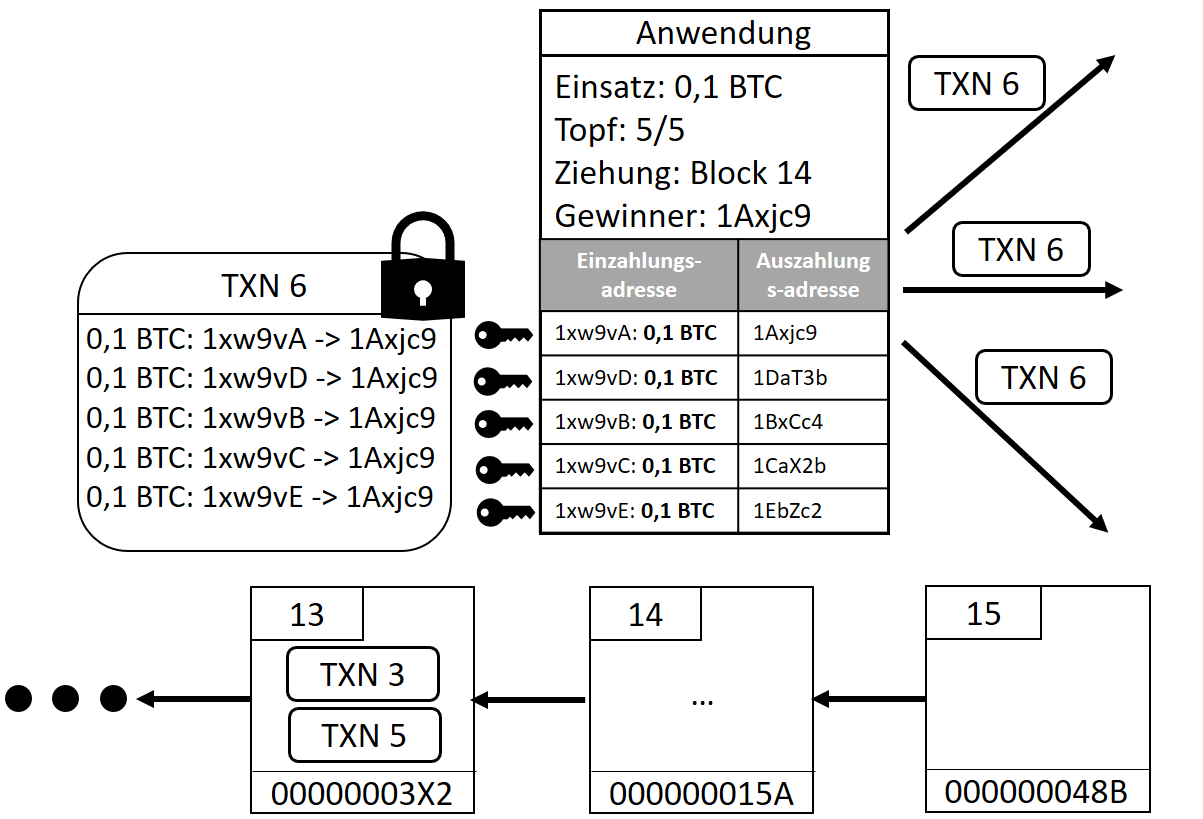
\includegraphics[width=\textwidth]{Figures/konzept_btc/konzept11}
\centering
\decoRule
\captionof{figure}{Schritt 11}
\label{fig:konzept11}
\end{minipage}
\begin{minipage}{0.45\textwidth}
Die Anwendung erstellt nun eine Transaktion, die alle Spieleinsätze an die Auszahlungsadresse \textbf{1Axjc9} von Spieler 1 überweist. Um die Transaktion zu signieren, verwendet die Anwendung die zu den 5 Einzahlungsadressen passenden privaten Schüssel. Anschließend leitet die Anwendung die Transaktion an das Peer-to-Peer Netzwerk weiter.
\end{minipage}

\vspace{1cm}
\begin{minipage}{0.55\textwidth}
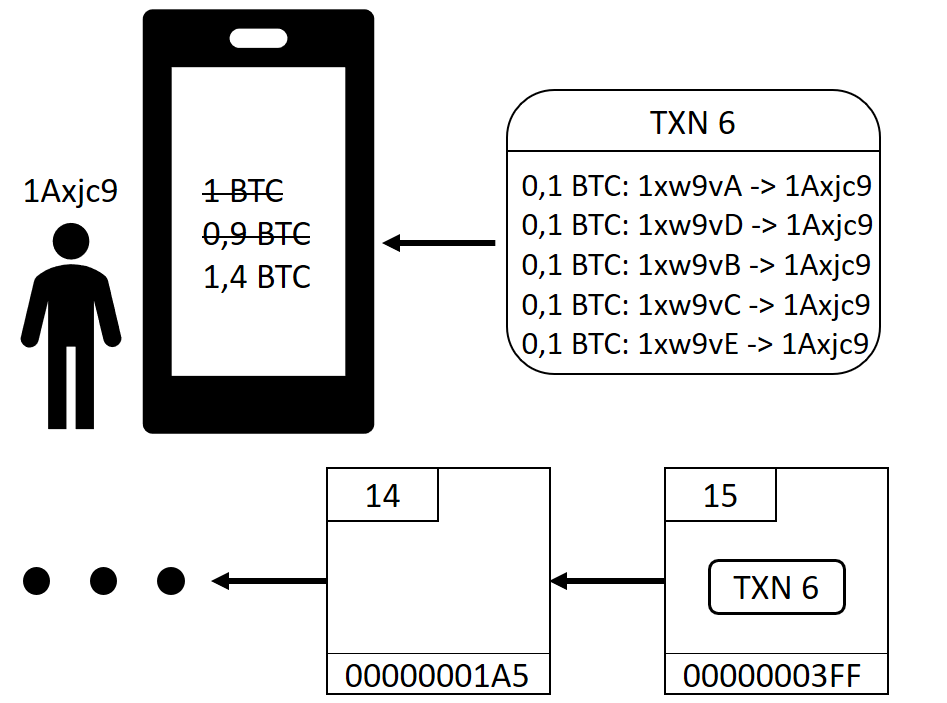
\includegraphics[width=\textwidth]{Figures/konzept_btc/konzept12}
\centering
\decoRule
\captionof{figure}{Schritt 12}
\label{fig:konzept12}
\end{minipage}
\begin{minipage}{0.45\textwidth}
Das Smartphone von Spieler 1 empfängt die Transaktion gegebenenfalls noch bevor sie von einem Miner in einen validen Block aufgenommen wurde. Die Wallet Software zeigt die Transaktion erst als unbestätigt an. Sobald sie durch die Aufnahme in Block 16 bestätigt wurde, gilt sie für die Wallet Software als bestätigt.
\end{minipage}